\documentclass[sigconf,12pt,review=false,natbib=false]{acmart}

\usepackage[style=ACM-Reference-Format,backend=bibtex,sorting=nty]{biblatex}
\addbibresource{research.bib}

\begin{document}

% ACM Format
\settopmatter{printacmref=false}
\setcopyright{none}
\renewcommand\footnotetextcopyrightpermission[1]{}
\pagestyle{plain}

%Title
\title{Bag of words with Naive Bayes to detect languages}

%Authors
\settopmatter{authorsperrow=2}

\author{Santiago E. Bocel}
\affiliation{%
    \institution{Universidad Rafael Landívar}
    \postcode{01016}
    \city{Guatemala City}
    \country{Guatemala}}
\email{santiagobocel10@gmail.com}

\author{Roberto Solares}
\affiliation{%
    \institution{Universidad Rafael Landívar}
    \postcode{01016}
    \city{Guatemala City}
    \country{Guatemala}}
\email{betosolaresgar@gmail.com}

\author{Brenner Hernandez}
\affiliation{%
    \institution{Universidad Rafael Landívar}
    \postcode{01016}
    \city{Guatemala City}
    \country{Guatemala}}
\email{velasquezbrenner@gmail.com}

\author{Pablo Muralles}
\affiliation{%
    \institution{Universidad Rafael Landívar}
    \postcode{01016}
    \city{Guatemala City}
    \country{Guatemala}}
\email{pablomuralles28@gmail.com}

% abstract
\begin{abstract}

Text classification also known as text tagging or text categorization is the process of categorizing
text into organized groups. By using Natural Language Processing (NLP), text classifiers can
automatically analyze text and then assign a set of pre-defined tags or categories based on its
content. \\

There are different types of text classifiers, for example, language detection, process automation,
virtual legislation, sentiment detection, etc. That is why the classification of texts is becoming
an increasingly important tool, since it allows us to obtain information from data and make use of
them quickly, something that is very important in the information age. \\

On the other hand, machine learning in its most basic form is the practice of using algorithms to
analyze data, learn from it, and then make a determination or prediction about something in the
world. Where there are endless techniques for learning, representation and optimization. \\

It is for these reasons that the combination of machine learning with text classification is a very
powerful but at the same time very complex tool and a field in which there is still much to
explore. \\

\end{abstract}

\maketitle

\section{Introduction}

Text classification is one of the applications of Machine Learning and consists of cataloging the
texts based on their content, that is, performing an analysis of the words to decide what type of
text is being identified. \\

This work is ideal for a machine as they are ideal for processing large amounts of information.
However, since the machine does not initially know how to catalog a text based on any criteria, it
requires a learning process in advance. \\

In this research, the Bag of Words (BOW) model will be used, which is a method used in language
processing to classify words according to the tag. \\

Many language processing tasks involve a classification, in which different machine learning methods
can be used such as Maximum Entropy (ME), Support Vector Machines (SVE), Naive Bayes (NB) and many
more, that is why that in this work the Naive Bayes algorithm was used, more specifically the
Gaussian Naive Bayes algorithm. The Gaussian Naive Bayes algorithm is of great help as it proposes a
solution to the categorization of text by assigning a label or a category to an entire text or
document. \\

All these methods and tools can be applied in different types of classifiers such as the
classification of feelings, which is the process of automating or identifying opinions in the text
and labeling them as positive, negative or neutral, based on the emotions or labels that it possesses.
each one, the spam classification of some text, the automatic generation of subtitles, among others.
In the case of this research, we focus on knowing the language in which a text is written, language
recognition. \\

This paper is structured as follows. The Fundamentals section describes the prior knowledge that the
reader is recommended to possess in order to have a better understanding of the research. In the
section The problem, the problem to be solved with this investigation is detailed as well as its
requirements. The Similar Implementations section describes which experiments and projects have
solved the same problem and how they have done it. In the section Our Solution, it is explained in
detail how the solution was carried out, as well as why certain decisions were made and what problems
were encountered when carrying out the same. The Results section describes what information could be
obtained both in the training phase as well as in the experimentation and testing phase. Finally, the
Conclusions section expresses the thoughts and observations of the authors after conducting the
research. \\

\section{Fundamentals}

\subsection{Artificial intelligence}

Its origins were in robotics but while this hardware was being made there was a need to create software that allows
this hardware to appear to have intelligence. Artificial intelligence seeks to be able to understand, perceive,
predict and to some extent be able to manipulate its environment. It has four approaches which are the following
systems that think like humans, systems that act like humans, systems that think rationally and systems that act
rationally. \\

Artificial Intelligence has different foundations such as the philosophy, mathematics, probability, economics,
neuroscience, communication and much more.
Computational engineering is the most important providing the artifact, that is, the computer and the software,
operating systems, the infinity of programming languages and the same tools to be able to generate applications.
Later the theory of control and cybernetics that shared the theory of control, cybernetics and the objective function.
And to finish the linguistics that computational linguistics contributed. \\

There are different branches of artificial intelligence such as: Robotics, strong AI, reasoning and decision
making, knowledge representation, planning, computer vision, machine learning, data mining, and language processing.

Machine learning and data mining consists of machines learning without having to be explicitly programmed for
that task by means of previous data. Language processing is how a computer can analyze audio and then convert it
to text for analysis. 


\subsection{Machine Learning}

It consists of machines learning without having to be explicitly programmed for a given task, relyng only on
previous data.
Some of the fundamentals for this branch are inferential statistics, computer science and pattern recognition.
Going deeper with statistics, Bayes' theorem is very important since it tells us the probability that an event will
occur given the knowledge of certain previous conditions related to this event.
Scientists investigated how to apply the biology of human neural networks to machines. This ended with the creation
of artificial neural networks, a computer model that is based on the way our neurons share information with each other
through a network of interconnected nodes. Following this, MIT Dean Edmonds and Marvin Minksy created a program
capable of learning through experience to get out of a maze. \\

Through inferential statistics, pattern recognition, and a sample of data, machine learning is able to draw inferences
from new data sets for which it has never been trained. It does this by performing large data analyzes in order to
deduce or infer which is the most optimal result for a certain situation. Taking into account that it has not been
designed or programmed to carry out this task, rather it generates a capacity to learn through data and it is here
where the step from programming through rules to autonomous learning is generated. \\

There are three main types of machine learning: supervised learning, unsupervised learning and reinforcement learning.
Supervised learning is when the agent is trained through data that is an example of the inputs and outputs that it
should have, that is, with data that is labeled. 
Unsupervised learning consists of learning through input patterns where the values for the outputs are not said,
it means that a specific type is not identified, but similarities are sorted and grouped. 
Finally, learning by effort, this is not taught with data but thanks to the environment that surrounds it and the
actions it takes, depending on its result, it learns.


\subsection{Joint and Conditional Probabilities}

The joint probability function describes the probability of two events occurring simultaneously. In
practice this is just the multiplication of the probabilities of all events. While the conditional
probability describes the probability of one event occurring in the presence of a second event. In
practice this is the multiplication of the probabilities of one event if the other event occurs and
the probability of the other event to occur. \\

As we can see, the joint probability and the conditional probability are basically equal, so they are
equivalent and we can denote it as follows.

\begin{figure}[h!]
    \centering
    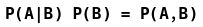
\includegraphics[]{jcp_relationship}
    \Description{Joint probability and conditional probability relationship}
    \caption{Joint and conditional probability}
    \label{fig:jcp_relationship}
\end{figure}

We can also express a joint probability in terms of chain of conditional probabilities and these are
known as the chain rule. \\

\begin{figure}[h!]
    \centering
    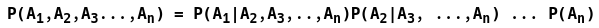
\includegraphics[width=4in]{chain_rule}
    \Description{Chain rule}
    \caption{Chain rule}
    \label{fig:jcp_relationship}
\end{figure}


\subsection{Statistical inference}

For an artificial intelligence to try to predict using some classification algorithm it must first learn its
probabilistic theories about the world from experience. 
Statistical inference is the induction that allows establishing a truth with a higher probability index than
the others. With this, artificial intelligence acquires a tool to solve specific problems, such as the classification
of information. \\

In Bayesian learning methods, learning is formulated as a form of probabilistic inference, using observations to
update a prior distribution on the hypothesis.
One simply calculate the probability of each hypothesis given the data, and make predictions on these samples.
This means that the predictions are made using all the hypothesis, weighted by their probabilities and not only
using the best of the hypothesis. In this way, learning is reduced to probabilistic inference.


\subsection{Bayes Theorem}

The Bayes theorem is used to calculate the probability of an event, having information in advance
about this event. In this way, it is possible to calculate the probability of an event A, also
knowing that the event A fulfills a certain characteristic that determines its probability. \\

Based on the above, it is understood that this branch of statistics is essential for the elaboration
of inference rules that can represent a viable way of learning for the way in which machines analyze
their results. \\

The Bayes theorem is attractive for artificial intelligence since it comes from the fact that its
development is axiomatic, allowing constructive growth based on a single derivation rule, so that by
significantly increasing the number of repetitions, there will be a perfectible improvement mechanism
which will represent the foundation for learning by repetition, erring less and less until reaching
an optimal knowledge of what is involved. \\


This theorem appear from the solving of the conditional probability equation, since we could see
that it is equivalent to the joint probability. \\

\begin{figure}[h!]
    \centering
    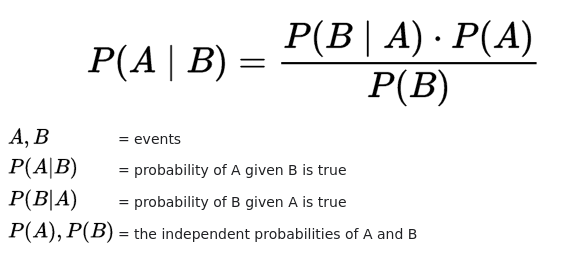
\includegraphics[width=3in]{bayes}
    \Description{Bayes theorem}
    \caption{Bayes theorem}
    \label{fig:jcp_relationship}
\end{figure}

\subsection{Naive Bayes}
Naive Bayes is a simple and powerful algorithm. Despite the significant advances in Machine Learning in recent
years, it has proven its worth. It has been successfully implemented in many applications, from text analysis
to recommendation engines. \\

It is one of the simplest and most powerful algorithms for classification based on Bayes' Theorem with an assumption
of independence between the predictors. It assumes that the effect of a particular feature on a class is independent
of other features. \\

Using the algorithm it is quick and easy to predict the kind of test data set. They also work well in multiclass
prediction. When the independence assumption is held, a Naive Bayes classifier performs better compared to other
models and less training data is required.
It works well for categorical input variables compared to numeric variables. \\

The disadvantages of using this algorithm are that if the categorical variable has a category in the test data set,
which was not observed in the training data set, the model assigns a probability of 0 and will not be able to make
a prediction. This is often known as the zero frequency. The smoothing technique can be used to solve this problem.
Another disadvantage is the assumption of independent predictors. In real life it is almost impossible for us to
obtain a set of predictors that are completely independent. \\

This algorithm serves a core part in our solution, wo we will talk more on how we implemented it.

\begin{figure}[h!]
    \centering
    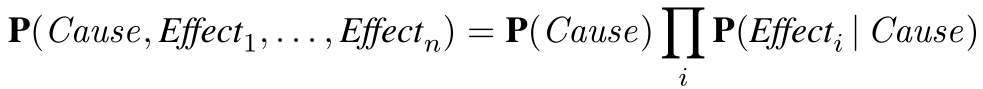
\includegraphics[width=3in]{naive_bayes}
    \Description{Naive Bayes}
    \caption{Naive Bayes}
    \label{fig:naive_bayes}
\end{figure}


\subsection{Bag of Words}

The Bag of Words is a method often used for document classification. This method turns text into fixed-length
vectors by simply counting the number of times a word appears in a document, a process referred to as vectorization. \\

Although these vectorization methods are easy to compute, it lacks any contextual information. It literally is a bag
of words – there is no order, it’s only the word counts that matter.
It is a data recovery system. It does the work of identifying all documents that are important for the user who
seeks the information. \\

\begin{figure}[h!]
    \centering
    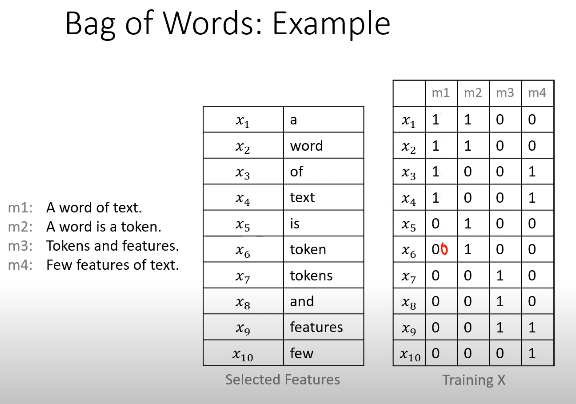
\includegraphics[width=3in]{bow}
    \Description{Bag of Words}
    \caption{Bag of Words}
    \label{fig:bow}
\end{figure}

This is also a core part of our project, thus, we will detail how our solution uses this algorithm.

\section{Our Problem}

We are four university students and are currently coursing our fourth year of computer engineering. In this semester
we enrolled to the Artificial Intelligence course, and so, we were assigned with this final project. We had to 
implemente the fist stage of a text classification system to identify languages through input text.
For this, we were appointed to use a Bag of Words system, in conjunction with a Bayesian model, more specifically,
Naive Bayes. \\

This implementation must support input text from files and user given phrases. These file inputs must follow a specific
structure; the first part of the input must be phrase in any language, the second part must be a name tag describing
the language in which that phrase was written; our solution will have to split this parts with a given separator,
in this case being a '|' (pipe character). Some examples could be: \\ 

\begin{description}
  \item[$\ast$] la vida empieza cada cinco minutos | español 
  \item[$\ast$] it is a good day to be happy | ingles
  \item[$\ast$] eu te quero com tudo meu coração | portugues \\ 
\end{description}

If the input is a user given phrase, we must be able to ask them for the corresonding name tag and associating each 
other.
The solution must process any given number of lines or phrases with any given number of labels. When inserting a new
line or phrase the solution must be readjusted. It must be taken into account that when reading a CSV file or similar,
the data should be normalized and cleaned. In addition, the solution must have a cold start option and at the time
of interaction with the user, the recommendations must improve. \\

The sofware had to be develped using any JVM compatible language, with the option of using any type of data base.


\section{Similar Implementations}

Another type of algorithms commonly used in automatic classification of texts are:

\subsection{Support vector machines(SVM)}

This algorithm is a text classification method. It corresponds to learning machines that take different characteristics
of the elements that want to classify and take them to a multidimensional vector space. It is in this space, where the
algorithm identifies a hyperphan that separates the vectors into a class different of the rest. \\

The solution for a Bag of Words classification is simple. Suppose that in the following image the blue dots represent
a language and the red dots other language, if a line is drawn between them, when there is a new point, we can say what
color is going to have, depending on the side of the line in which you are. \\

\begin{figure}[h!]
    \centering
    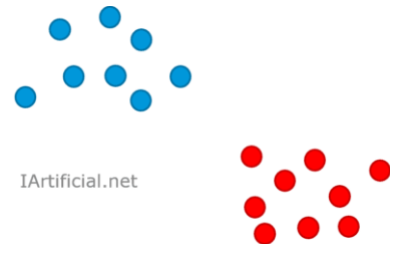
\includegraphics[]{svm}
    \Description{Support vector machine}
    \caption{Support vector machine}
    \label{fig:svm}
\end{figure}

The line that best separates the zone of the blue dots from the red dots area is the line that maximizes the margin
between them. Support vector machines are a Machine Learning technique that finds the best possible separation between
classes. With two dimensions it is easy to understand what you are doing. Normally, automatic learning problems have a
lot of dimensions. So instead of finding the optimal line, the SVM finds the hyperphan that maximizes the margin of
separation between classes.

\subsection{K-nearest neighbors algorithm (KNN)}

This is a learning algorithm based on supervised type instances of Machine Learning. It is used to classify new samples
or to predict. It is a simple method, looks for the closest observations to which you are trying to predict and classify
the point of interest based on most data that surrounds it. \\

The solution for a Bag of Words classification is also simple.
The distance between the word to classify and the rest of the words of the training dataset should be calculated. Then
select the closest elements (with less distance, according to the function that is used). Finally, perform a "majority
vote" between the K points: those of a class / dominant label will decide its final classification.



\section{Our Solution}

In a way or another, we used all of the information previously exposed to acomplish this solution for the given problem.
We developed a Bag of Words with Naive Bayes using the Java programming language.

The interaction that the user will have with our solution will be through the command line. They will be presented
with a series of menus, firstly they will see the main menu:

\begin{figure}[h!]
    \centering
    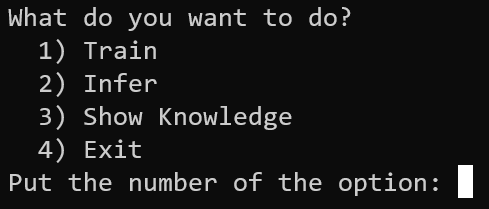
\includegraphics[]{main_menu}
    \Description{Main menu}
    \caption{Main menu}
    \label{fig:main_menu}
\end{figure}

\section{Results}


\section{Conclusions}

\begin{description}
    \item[$\bullet$] One of the greatest advantages of Naive Bayes over other classification algorithms is its ability
      to process an extremely large amount of data. \\
  \item[$\bullet$] The Naive Bayes algorithm is simple to implement, works well from the beginning and adjusting its
      parameters is rarely necessary. \\
  \item[$\bullet$] Even though Naive Bayes has great advantages, a smoothing technique to prevent probabilities to be
      zero was necessary. \\
  \item[$\bullet$] Considering the amount of data they can handle, the training and process of prediction are very
      fast even when they start cold. \\
  \item[$\bullet$] Automatic learning was specifically applied to the supervised learning branch. \\
\end{description}

% References
\nocite{*}
\printbibliography

\end{document}
